%\begin{flushright}
%\end{flushright}
\documentclass{template/openetcs_report}
% Use the option "nocc" if the document is not licensed under Creative Commons
%\documentclass[nocc]{template/openetcs_article}
\usepackage{lipsum,url}
\usepackage{supertabular}
\usepackage{multirow}
\usepackage{color, colortbl}
\usepackage{float}
\definecolor{gray}{rgb}{0.8,0.8,0.8}
\usepackage[modulo]{lineno}
\graphicspath{{./template/}{.}{./images/}}


%=======================================================================
%%%%% comments %%%%%
% To allow MS Word style comments at the document margin we use the todonotes package. A comment is made as follows:

%\mycomment[IN]{text}

% The text in brackets should be your initials and the text in curly braces is your actual comment. Comments are numbered automatically. 
\usepackage[textwidth=2.7cm,textsize=scriptsize,linecolor=green!40,backgroundcolor=green!40]{todonotes}

\newcounter{mycommentcounter}
\newcommand{\mycomment}[2][]
{
\refstepcounter{mycommentcounter}%
\todo[color={red!100!green!33}]{
\textbf{[\uppercase{#1} \themycommentcounter]:} #2}
}
\setlength{\marginparwidth}{2.5cm}
%\reversemarginpar
%=======================================================================


\begin{document}
\frontmatter
\project{openETCS}

%Please do not change anything above this line
%============================
% The document metadata is defined below

%assign a report number here
\reportnum{OETCS/WP2/?}

%define your workpackage here
\wp{Work-Package 2}

%set a title here
\title{Scrum Process in openETCS Project}

%set a subtitle here
\subtitle{}

%set the date of the report here
\date{August 2015} % \\ Revised April 2015}

%document approval
%define the name and affiliation of the people involved in the documents approbation here
\creatorname{Abdelnasir Mohamed}
\creatoraffil{AEbt}

\techassessorname{}
\techassessoraffil{}

\qualityassessorname{}
\qualityassessoraffil{}

\approvalname{Klaus-R\"udiger Hase}
\approvalaffil{DB Netz}

%define a list of authors and their affiliation here

\author{Abdelnasir Mohamed}

\affiliation{AEbt Angewandte Eisenbahntechnik GmbH\\
  Adam-Klein-Str. 26 \\
  90429 Nürnberg, Germany\\
  eMail: abdelnasir.mohamed@aebt.de \\
  WebSite: www.aebt.de}  

\author{Jan Welte}

\affiliation{Technische Universität Braunschweig\\
  Institute for Traffic Safety and Automation Engineering\\
  Hermann-Blenk-Str. 42\\
  38108 Braunschweig, Germany\\
  eMail: openetcs@iva.ing.tu-bs.de \\
  WebSite: www.iva.ing.tu-bs.de}
  

%add yourself as author, if you contributed to the document



% define the coverart
\coverart[width=350pt]{openETCS_EUPL}

%define the type of report
\reporttype{Output Document}


\begin{abstract}

\end{abstract}

%=============================
%Do not change the next three lines
\maketitle
\tableofcontents
\listoffiguresandtables
\newpage
%=============================

\chapter{Document Control}

\begin{tabular}{|p{4.4cm}|p{8.7cm}|}
\hline
\multicolumn{2}{|c|}{Document information} \\
\hline
Work Package &    \\
Deliverable ID & \\
\hline
Document title & openETCS \\
Document version & 01.1 \\
Document authors (org.)  & Jan Welte (TU-BS) and Abdelnasir Mohamed (AEbt)\\
\hline
\end{tabular}

\begin{tabular}{|p{4.4cm}|p{8.7cm}|}
\hline
\multicolumn{2}{|c|}{Review information} \\
\hline
Last version reviewed & 0.1 \\
\hline
Main reviewers (org.) & \\
\hline
\end{tabular}

\begin{tabular}{|p{2.2cm}|p{4cm}|p{4cm}|p{2cm}|}
\hline
\multicolumn{4}{|c|}{Approbation} \\
\hline
  &  Name & Role & Date   \\
\hline  
Written by    &  Jan Welte & WP4-T4.4 Task Leader  &  March 2015\\
\hline
Approved by & -- & -- & \\
\hline
\end{tabular}

\begin{tabular}{|p{2.2cm}|p{2cm}|p{4cm}|p{4cm}|}
\hline
\multicolumn{4}{|c|}{Document evolution} \\
\hline
Version &  Date & Author(s) & Justification  \\
\hline
0.1 & 18/08/2015 & Jan Welte &  Document creation \\
\hline 
0.2 & 19/10/2015 & Abdelnasir Mohamed & Chapter 1.1 \\
\hline  
00.1 & 28/01/2014 &  &   \\

\hline  
\end{tabular}
\newpage

%=========ToDo List===========
\listoftodos[ToDo List]
\newpage
% The actual document starts below this line
%=============================

\mainmatter

\chapter{Introduction}
\label{sec:introduction}
 
Nasir

Short introduction to this document.
\mycomment[AM]{Introduction: finish section writing}
\begin{itemize}
\item extension to QA-Plan and Process Description
\end{itemize}



\section{Purpose}
\label{sec:purpose}

The purpose of this document is to define and describe the agile work-flow of the software development process in the openETCS project. As the outcomes of the project, the openETCS software and the openETCS development Tool chain, are precisely defined, the process of how these two artifacts at the beginning of the development process are being produced in detail is not clear. In the conventional software development  process, e.g. with a V-Model, the life cycle of the development is implemented in closed non re-definable phases, which they shall be processed consecutively. 

Due to the complex nature of the openETCS as a  Research and Development (R\&D) Project an agile methodology is needed, which it's framework facilitates continuous refinements and improvements throughout the whole openETCS software development process. In this agile way of development complex Tasks are broken down into smaller Tasks (increments), which shall be executed in short time frames called Sprints. This document will be describing the agile framework in openETCS development process applying SCRUM.


%\section{Document Structure}
%\label{sec:document-structure}



%\section{Document Evolution}



\section{Reference Documents}
\label{sec:refdoc}

This document essentially refers to the following standards, ETCS specification documents and openETCS project documents.

\begin{itemize}
\item \textbf{ISO~9000} --- 12/2005 --- \emph{Quality management}
\item \textbf{ISO~9001} --- 12/2008 --- \emph{Quality management systems — Requirements}
\item \textbf{ISO~25010} --- 03/2011 --- \emph{Systems and software engineering -- Systems and software Quality Requirements and Evaluation (SQuaRE) -- System and software quality models}
\item \textbf{CENELEC EN~50126-1} --- 01/2000 --- \emph{Railways applications –- The specification and 
demonstration of Reliability, Availability, Maintenability and Safety (RAMS) –- Part 1: 
Basic requirements and generic process}
\item \textbf{CENELEC EN~50128} --- 10/2011 --- \emph{Railway applications -- Communication, signalling and 
processing systems -- Software for railway control and protection systems}
\item \textbf{CENELEC EN~50129} --- 05/2003 --- \emph{Railway applications –- Communication, signalling and 
processing systems –- Safety related electronic systems for signalling}
\item \textbf{CCS~TSI} --- \emph{ CCS TSI for HS and CR transeuropean rail has been adopted by a Commission Decision 2012/88/EU on the 25th January 2012}
\item \textbf{SUBSET-026} 3.3.0 --- \emph{System Requirement Specification}
\item \textbf{SUBSET-091} 3.2.0 --- \emph{Safety Requirements for the Technical Interoperability
of ETCS in Levels 1 \& 2}
\item \textbf{SUBSET-088} 2.3.0 --- \emph{ETCS Application Levels 1 \& 2 - Safety Analysis}
\item \textbf{OpenETCS FPP} --- \emph{Project Outline Full Project Proposal Annex OpenETCS} -- v2.2
\item \textbf{OpenETCS D2.2} -- Report on CENELEC standard
\item \textbf{OpenETCS D2.3} -- Definition of the overall process for the formal description of ETCS and the rail system it works in 
\item \textbf{OpenETCS D2.4} -- Definition of the methods used to perform the formal description
\item \textbf{The Scrum Guide} -- The Definitive Guide to Scrum: The Rules of the Game, July 2013
\end{itemize}


%%%%%%%%%%%%%%%%%%%%%%%%%%%%%%%%%%%%%%%%%%%%%%%%%%%%%%%%%%%%%%%

\section{Glossary}
\label{sec:glossary}



\begin{tabular}{rl}
\textbf{ACedit} & Assurance Case Editor \\ 
\textbf{ARM} & Argumentation  Metamodel \\ 
\textbf{ETCS} & European Train Control System \\ \textbf{ERA} & European Railway Agency \\ \textbf{FMEA} & Failure Mode Effect Analysis \\ 
\textbf{GSN} & Goal Structured Notation \\ 
\textbf{MoRC} & Management of Radio Communication \\ 
\textbf{RAMS} & Reliability, Availability, Maintainability and Safety \\
\textbf{SIL} & Safety Integrity Level \\ 
\textbf{SRS} & System Requirement Specification \\ 
\textbf{THR} & Tolerable Hazard Rate \\ 
\textbf{V\&V} & Verification \& Validation \\ 
\end{tabular} 




\section{Background Information}
\label{sec:Background}


\subsection{Agile Development}

Jan

really short introduction to the concept of agile development overall
\mycomment[AM]{Agile Development: finish section writing}

\subsection{SCRUM Definition And Roles}

This section should be considered as an introduction for the following chapters to fit the content of this document. For more detailed information about SCRUM the \textit{Scrum Guide} is advisable to read. In the SCRUM Guide developed by Ken Schwaber and Jeff Sutherland, Scrum is defined as "\textit{A framework within which people can address complex adaptive problems, while productively and creatively delivering products of the highest possible value}". It is "\textit{simple to understand}" but "\textit{difficult to master}".

SCRUM defines three roles; the Product Owner (PO); the SCRUM Master (ScM) and the Development Team. All three roles together make the SCRUM Team.

\subsection{General SCRUM Framework}

Scrum process starts with a Product Backlog (PB), this Product Backlog contains an ordered list of requirements that is maintained for a product. The Product Backlog Items (PBIs) are ordered by the Product Owner based on considerations like risk, business value, date needed, etc. The Product Owner is the responsible of the product backlog and the prioritization of PBIs.

After the defining of the Product Backlog the next task is to create the Sprint planning meeting. This meeting is organized at the beginning of the Sprint cycle. The objective of this meeting is to define the PBIs to be done in following Sprint. The Sprint is the time period in which development occurs on a set of backlog items that the team has committed to (also commonly referred to as iteration). 

The result of PBIs selected for implementation in one Sprint is called the Sprint Backlog. The Sprint Backlog is the list of work the Development Team must address during the next Sprint. This list is derived by selecting product backlog items from the top of the product backlog until the Development Team fills it's capacity and make sure it has enough work to during the CompSprint.

Each day during the Sprint, a project team communication meeting occurs. This is called a daily Scrum Meeting and has specific guidelines. The Scrum Meeting is organized by the Scrum Master and the participants respond to three questions:
\begin{enumerate}
\item  What have you done since yesterday?
\item What are you planning to do today? 
\item And Any impediments/stumbling blocks?.
\end{enumerate}
At the end of the Sprint, the result of the PBIs implemented is called the increment (potentially shippable increment), this is the sum of all the Product Backlog items completed during a Sprint and all previous Sprints. The increment must be in a usable condition regardless of whether the Product Owner decides to actually release it.

At the end of Sprint cycle or iteration, two meetings are held; the Sprint review meeting and Sprint retrospective. The approximate duration of the spring review meeting will be no more than 4 hours and it will be moderated by the Scrum Master (ScM). In this meeting two main activities will take place. One is to review the the planned work that has been completed from the one that wasn't. And the second activity is to present to the Product owner the work done. The other meeting after iteration is the spring retrospective. This meeting will be moderated by the scrum master and it's main objective is the continuous process improvements. Two main questions are asked to all participants in this meeting:
\begin{itemize}
\item   what went well during the Sprint? 
\item What could be improved in the next Sprint?? 
\end{itemize}


\chapter{Agile Development in openETCS}
\label{sec:agile}

Jan
\reversemarginpar
\mycomment[AM]{Agile Dev oETCS: finish section writing}

Basic concept of agile development in openETCS.
Allocation of agile work principles to 

\begin{itemize}
\item allocating agile work activities to the iterative work in openETCS development life cycle (phases nd artifacts) 
\item describe overlap between EN 50128 roles and Scrum roles
\end{itemize}



\chapter{openETCS SCRUM Process}
\label{sec:ScrumProzess}

In openETCS there are three levels of processes that apply SCRUM:
\begin{itemize}
	\item The first level is the openETCS Project level, where Project Coordinator is the Product Owner. In this level the SCRUM meetings are organized every Friday.
	\item The second level is the Work Package level, where Work Package Leader is the Product Owner. In this level SCRUM meeting depends on WP, but at least two SCRUM meetings are organized every week.
	\item The last level is the Task level, where the Task Leader is the Product Owner. In this level SCRUM meeting period is variable and depends on the task.
\end{itemize}

\begin{figure}[h]
	\centering
	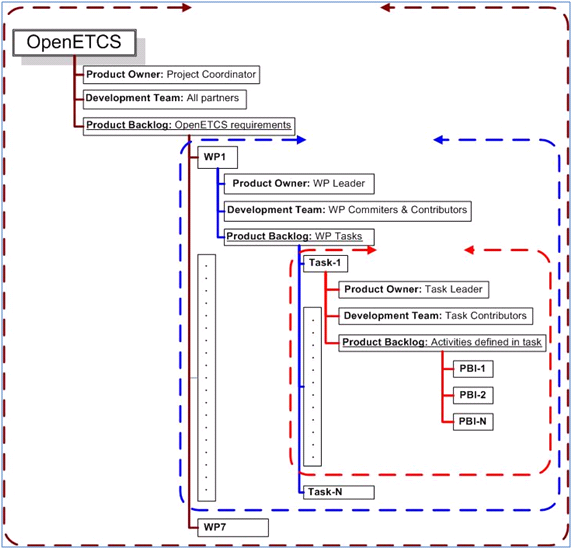
\includegraphics[scale=0.6]{./images/openetcs__scrum.png}
	\caption{openETCS Project Structure}
\end{figure}

\mycomment[AM]{finish section writing} \\

\section{SCRUM Process in Work Packages}

- As defined in FPP there are 7 WPs\\
- WP Roles and it's conventions to conform the EN 50128 Roles\\
- Grafik of Roles for SW dev. in EN 50128 
- Every WP has its own PO\\
- Webbased CM (GitHub)\\
-----------------------------------------


\textbf{Product backlog of the Modeling Team (WP3)}

The product backlog is implemented via the issue tracker.
The product backlog consists ofUse Cases, marked with the label "US-Operational Scenarios on Utrecht Amsterdam".
Each Use Cases has an unique User Story label identifing this Use Case in the backlog.
(Sub-) User Stories identified as necessary for the implementation of a Use Cases are marked with the user story label,

The actual work at the user stories is broken down in smaller technical tasks. These tasks are organised in the sprint backlog. Use the label sprint backlog for defining a task.
Remark: We will use specific sprint labels when we better start to organise the work in individual sprints.

The sprint backlog consists of prioritized tasks. Priorities are integers in the interval [1...1000], with 1000 representing the highest priority. Note that the absolute value is of minor interest, priorization is only needed to classify backlog items by importance.

Priorities are captured in the title of each task respectively issue. Example: US-SpeedMonitoring: Dynamic ASave Calculation Prio: 500 represents a user story with priority 500. The reason to capture the priority in the title is to make priority changes traceable, as the text of github issues may be changed without leaving any trace.

The labels Ready, In Progress, and Deferred are used to capture the state of user stories. Note that closing an issue is equivalent to the state Done.

A user story may only be moved to the state Ready when:
	A priority has been assigned.
	The scope is clearly defined and distinguished from other user stories in the states Ready or in Progress.
	The criteria for reaching the state Done are clear.
	When setting a user story to "done" a comment is mandatory for documenting the result.
	Every project member is eligible to propose user stories.

New user stories shall remain in the state (respectively column) Inbox until they have been reviewed by the team in a grooming session. 





\missingfigure{SCRUM in WPs} \\ \\


%mycomment{} have been wrongly placed on the left margin

Here!
\reversemarginpar
\mycomment[AM]{SCRUM in WPs GitHub: finish section writing}

\section{Scrum of Scrums}


Nasir

Short introduction to principle of splitting work between different teams, as required by the EN 50128

Principles of grooming work and filling backlogs for distributed Scrum Teams by dynamic work allocation.

Text based on wiki page by Marc Behrens
\mycomment[AM]{SCRUM of SCRUMS Wiki in WP3 GitHub: finish section writing}
\textit{Objective:} Ongoing verification and validation of openETCS development artifacts are performed within the framework of openETCS scrum process. This page describes the interface of agile verification and validation to the top level customer as well as the scrum process within the verification and validation itself.

\begin{figure}[h]
\centering
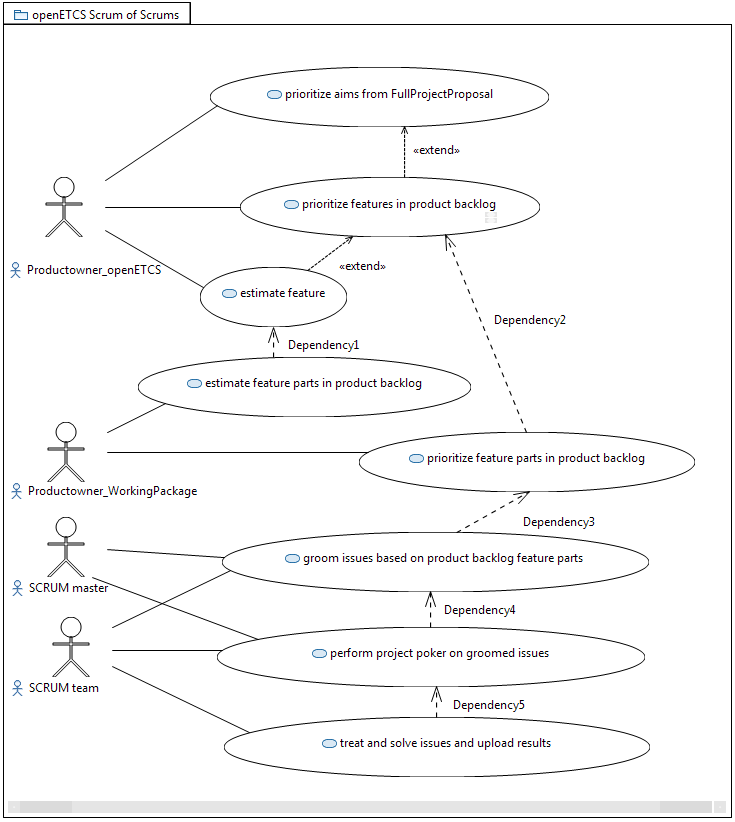
\includegraphics[width=0.7\linewidth]{./images/openETCSVnVScrumOfScrum_02}
\caption{openETCS scrum of scrums}
\label{fig:openETCSVnVScrumOfScrum}
\end{figure}

Within the agile scrum process of openETCS different backlogs are used to synchronise the top level project goals with the tasks performed within the project: 

\begin{itemize}
\item Each backlog itself consists of items which are represented within the github issue tracker. 
\item For each backlog a Product Owner is assigned to coordinate and prioritize the items.
\item Each Story Point (SP) is estimated to be worth one person day.
\end{itemize}


\textbf{The Product Backlog (Product Owner: Klaus-Rüdiger Hase)}
The Product Backlog consists of top level \textit{Features} by which the product is described.
\begin{itemize}
\item  Each Feature itself is estimated by the product owner on how many Story Points this Feature is worth.
\item  A Feature itself is divided into **Feature Parts**.
\item  A Feature Part is related directly to a working package and the repository the work is documented in.
\item  Each Feature Part itself is estimated and prioritized by the product owner on how many Story Points this Feature Part is worth.
\end{itemize}


By estimating the feature the feature becomes accepted on product Level.
The Product Backlog is maintained during a regular meeting.

\textbf{Transferring the Features from the \textit{Product Backlog} to the Verification and Validation Sprint Backlog}
During regular grooming sessions the scrum team extracts the items with highest priority out of the Product Backlog and refines them to issues within the repository mentioned within the Feature Part.
On these issues Project Poker is performed on and by this Story Points are assigned. The decision on which items enter the Sprint Backlog is based on the maximum benefit analysis taking into account the priority as well as the story points.

\textbf{Sprint Backlog}
The \textit{Sprint Backlog} consists of issues which are processed during the Sprint.
During the Sprint the success is tracked against the Sprint Backlog.
The Story Points are earned once the complete result of what has been groomed is uploaded to the github.

\chapter{Release Principals}
\label{sec:Releases}

Jan

principles of artifact releases (specially models) and their verification and validation
configuration management of design artifacts, test specifications and test reports
change management via issues, status of documents, criteria for releases and assessment


\chapter{Conclusion}
\label{sec:conclusion}

can be left open for now

final conclusion of content 


%\bibliographystyle{unsrt} %
%\bibliography{./ref/ref-HaRA}


%===================================================
%Do NOT change anything below this line

\end{document}


